\id{МРНТИ 81.93.25}{https://doi.org/10.58805/kazutb.v.4.25-669}

\begin{articleheader}
\sectionwithauthors{А.М. Курманов, А.Б. Бекмагамбетов, И.Е. Сарыбаева, А.Р. Енсебаева, А.Н. Омаркожаева}{РОЛЬ ЧЕЛОВЕКОЦЕНТРИЧНОГО ПОДХОДА В МОДЕРНИЗАЦИИ СОЦИАЛЬНЫХ
ГАРАНТИЙ ДЛЯ РАБОТНИКОВ ВО ВРЕДНЫХ УСЛОВИЯХ}

{\bfseries \textsuperscript{1}А.М. Курманов, \textsuperscript{1}А.Б.
Бекмагамбетов, \textsuperscript{2}И.Е. Сарыбаева,
\textsuperscript{1}А.Р. Енсебаева\textsuperscript{\envelope },}
{\bfseries \textsuperscript{1}А.Н. Омаркожаева}
\end{articleheader}
\begin{affiliation}

\textsuperscript{1}Республиканский научно-исследовательский институт по
охране труда Министерства труда и социальной защиты населения Республики Казахстан, Астана,
Казахстан,

\textsuperscript{2}Евразийский национальный университет им. Л.Н. Гумилева, Астана, Казахстан

\raggedright{\bfseries \textsuperscript{\envelope }}Корреспондент-автор: nel1212@gmail.com
\end{affiliation}

В статье проводится анализ существующей системы социальных гарантий для
работников, занятых во вредных и опасных условиях труда в Республике
Казахстан. Основное внимание уделено проблемам, связанным с
недостаточной эффективностью мер социальной поддержки и ограниченностью
традиционных методов компенсации вредных факторов. Рассматривается
концепция человекоцентричного подхода, направленного на повышение
качества жизни и безопасности работников.

На основе анализа статистических данных и обзора текущего
законодательства выявлены ключевые недостатки системы, включая
отсутствие индивидуализированного подхода и низкий уровень профилактики
профессиональных заболеваний. В работе предлагаются направления
модернизации социальных гарантий, такие как усиление профилактических
мер, внедрение цифровых технологий для мониторинга здоровья работников и
разработка программ реабилитации. Особое внимание уделяется роли
человекоцентричного подхода в улучшении условий труда и снижении уровня
профессиональных рисков.

В статье предложены рекомендации по переходу к гибкой и ориентированной
на человека системе социальной защиты, что, по мнению авторов, позволит
создать более безопасные и справедливые условия труда, повысить
удовлетворенность работников и снизить уровень производственного
травматизма и заболеваний.

{\bfseries Ключевые слова:} социальные гарантии, человекоцентричный подход,
охрана труда, вредные условия труда, профессиональные заболевания,
производственный травматизм
\begin{articleheader}

{\bfseries ЗИЯНДЫ ЖАҒДАЙЛАРДА ЖҰМЫСШЫЛАР ҮШІН ӘЛЕУМЕТТІК КЕПІЛДІКТЕРДІ
ЖАҢҒЫРТУДАҒЫ АДАМҒА БАҒЫТТАЛҒАН ТӘСІЛДІҢ РӨЛІ}

{\bfseries \textsuperscript{1}А.М. Курманов, \textsuperscript{1}А.Б.
Бекмагамбетов, \textsuperscript{2}И.Е. Сарыбаева,
\textsuperscript{1}А.Р. Енсебаева\textsuperscript{\envelope },}
{\bfseries \textsuperscript{1}А.Н. Омаркожаева}
\end{articleheader}
\begin{affiliation}

\textsuperscript{1}Қазақстан Республикасы Еңбек және халықты әлеуметтік
қорғау министрлігінің Еңбекті қорғау жөніндегі республикалық
ғылыми-зерттеу институты, Астана, Қазақстан,

\textsuperscript{2}Л. Н. Гумилев атындағы Еуразия ұлттық университеті, Астана, Қазақстан,

e-mail:nel1212@gmail.com
\end{affiliation}

Мақалада Қазақстан Республикасында зиянды және қауіпті еңбек
жағдайларында жұмыс істейтін қызметкерлер үшін қолданыстағы әлеуметтік
кепілдіктер жүйесіне талдау жүргізіледі. Әлеуметтік қолдау шараларының
тиімділігінің жеткіліксіздігіне және зиянды факторларды өтеудің дәстүрлі
әдістерінің шектелуіне байланысты проблемаларға басты назар аударылады.
Қызметкерлердің өмір сүру сапасы мен қауіпсіздігін арттыруға бағытталған
адамға бағытталған тәсіл тұжырымдамасы қарастырылуда.

Статистикалық деректерді талдау және ағымдағы заңнаманы шолу негізінде
жүйенің негізгі кемшіліктері, соның ішінде жекелендірілген тәсілдің
болмауы және кәсіптік аурулардың алдын алудың төмен деңгейі анықталды.
Жұмыста алдын алу шараларын күшейту, қызметкерлердің денсаулығын
мониторингілеу үшін цифрлық технологияларды енгізу және оңалту
бағдарламаларын әзірлеу сияқты әлеуметтік кепілдіктерді жаңғырту
бағыттары ұсынылады. Еңбек жағдайларын жақсартудағы және кәсіптік
тәуекелдер деңгейін төмендетудегі адамға бағытталған тәсілдің рөліне
ерекше назар аударылады.

Мақалада икемді және адамға бағытталған әлеуметтік қорғау жүйесіне көшу
бойынша ұсыныстар ұсынылған, бұл авторлардың пікірінше, қауіпсіз және
әділ еңбек жағдайларын жасауға, қызметкерлердің қанағаттануын арттыруға
және өндірістік жарақат пен аурудың деңгейін төмендетуге мүмкіндік
береді.

{\bfseries Түйін сөздер:} әлеуметтік кепілдіктер, адамға бағытталған тәсіл,
еңбекті қорғау, зиянды еңбек жағдайлары, кәсіптік аурулар, өндірістік
жарақаттану.
\begin{articleheader}

{\bfseries THE ROLE OF A HUMAN-CENTRED APPROACH IN MODERNISING SOCIAL
GUARANTEES FOR WORKERS IN HAZARDOUS CONDITIONS}

{\bfseries \textsuperscript{1}A.M. Kurmanov, \textsuperscript{1}A.B.
Bekmagambetov, \textsuperscript{2}I.E. Sarybaeva,
\textsuperscript{1}A.R. Yensebayeva\textsuperscript{\envelope },}
{\bfseries \textsuperscript{1}A.N. Omarkozhaeva}
\end{articleheader}

\begin{affiliation}

\textsuperscript{1}Republican Research Institute for labor protection of
the Ministry of Labor and social protection of the population of the
Republic of Kazakhstan, Astana, Kazakhstan,

\textsuperscript{2}L.N. Gumilyov Eurasian National University, Astana,

e-mail:\href{mailto:nel1212kz@gmail.com}{\nolinkurl{nel1212kz@gmail.com}}
\end{affiliation}

The article analyzes the existing system of social guarantees for
workers employed in harmful and dangerous working conditions in the
Republic of Kazakhstan. The main attention is paid to the problems
associated with the insufficient effectiveness of social support
measures and the limitations of traditional methods of compensating for
harmful factors. The concept of a human-centered approach aimed at
improv\-ing the quality of life and safety of employees is considered.

Based on the analysis of statistical data and a review of current
legislation, key shortcomings of the system have been identified,
including the lack of an individualized approach and a low level of
prevention of occupational diseases. The paper suggests areas for the
modernization of social guarantees, such as strengthening preventive
measures, the introduction of digital technologies for monitoring the
health of workers and the development of rehabilitation programs.
Special attention is paid to the role of the human-centered approach in
improving working conditions and reducing occupational risks.

The article offers recommendations on the transition to a flexible and
human-oriented social protection system, which, according to the
authors, will create safer and fairer working conditions, increase
employee satisfaction and reduce the level of occupational injuries and
diseases.

{\bfseries Keywords:} social guarantees, human-centered approach, labor
protection, harmful working conditions, occupational diseases,
industrial injuries
\begin{multicols}{2}

{\bfseries Введение.} В современном Казахстане вопросы социальной защиты
работников, занятых во вредных и опасных условиях труда, приобретают
первостепенное значение. На фоне экономических и социальных изменений
государство и бизнес осознают необходимость не только обеспечения
базовых социальных гарантий, но и создания более гибкой и
ориентированной на человека системы поддержки. В ответ на этот вызов
Концепция развития государственного управления в Республике Казахстан до
2030 года провозглашает переход к сервисной и «человекоцентричной»
модели управления, где во главу угла ставятся потребности граждан и их
благополучие {[}1{]}. Данный подход также отражен в ряде международных
стандартов, например, в Руководстве Международной организации труда по
системам управления охраной труда (ILO-OSH 2001) подчеркивается, что
безопасность и здоровье работников должны быть приоритетом на всех
уровнях трудового процесса, с акцентом на вовлеченность сотрудников в
разработку и реализацию мер по снижению профессиональных
рисков\hspace{0pt}.

Стандарт ISO 45001:2018 дополняет эту концепцию, вводя понятие
вовлеченности работников как центрального элемента системы охраны труда.
В документе отмечено, что работодатели обязаны не только минимизировать
риски, но и активно привлекать работников к процессу принятия решений о
безопасности, создавая условия для их непосредственного
участия\hspace{0pt}. Эти подходы служат основой для разработки
человекоцентричных моделей социальной защиты, которые включают как
компенсационные меры, так и превентивные инициативы.

Человекоцентричный подход к управлению, особенно актуальный для систем
социальных гарантий, означает фокус на личности как на основном объекте
и субъекте всех социальных и трудовых процессов. Этот принцип выдвигает
на первый план здоровье, безопасность, профессиональное развитие и
удовлетворенность каждого сотрудника. Он предполагает не просто
выполнение формальных обязательств, но глубокую заботу о благосостоянии
работников, особенно тех, кто ежедневно сталкивается с рисками для
здоровья и жизни.

В настоящее время понятие «человекоцентричная модель социальных
гарантий» не имеет единого общепринятого определения. Однако в ряде
научных исследований и работ рассматривается применение
человекоцентричных подходов в различных областях, включая управление
персоналом, социальные гарантии и модели развития экономики. Например, в
статье Гальченко С.А. и др. {[}2{]} отмечается, что человекоцентричность
является ключевым элементом экономики будущего, фокусируясь на
индивидуальных потребностях, развитии человеческого потенциала и
гармонизации отношений между технологиями и людьми\hspace{0pt}. В трудах
Абдешова Д.Д. и коллег {[}3{]} выделяются особенности
человекоцентричного управления человеческими ресурсами, в основе
которого лежит гуманизация труда и создание условий для раскрытия
интеллектуального и психологического потенциала работников.
Аналогичные подходы подчеркиваются в исследованиях, посвященных
корпоративным моделям, где человекоцентричность способствует повышению
удовлетворенности и вовлеченности сотрудников, что, в свою очередь,
повышает эффективность работы организаций\hspace{0pt}\hspace{0pt}.

Традиционные методы социальной защиты, применяемые в Казахстане,
включают:

\begin{itemize}
\item
  дополнительные выплаты за работу во вредных условиях;
\item
  сокращенное рабочее время для работников на опасных производствах;
\item
  дополнительные отпуска для восстановления здоровья;
\item
  обеспечение лечебно-профилактическим питанием для снижения воздействия
  вредных факторов\hspace{0pt}\hspace{0pt}.
\end{itemize}

Эти меры, хотя и доказали свою эффективность в прошлом, требуют
обновления в контексте современных вызовов и необходимости внедрения
человекоцентричных подходов. Например, в концепции управления
человеческими ресурсами акцент смещается с компенсации ущерба на
профилактику профессиональных заболеваний и создание безопасной среды
труда\hspace{0pt}\hspace{0pt}.

Человекоцентричная модель социальных гарантий предлагает революционное
переосмысление подхода к социальной защите. Она призвана интегрировать
принцип заботы о человеке в каждый элемент системы социальной поддержки.
Такой подход ориентируется на создание устойчивых условий труда,
снижение профессиональных рисков и заботу о здоровье работников, а также
на вовлечение самих сотрудников в процесс формирования системы
социальной защиты. Внедрение подобной модели требует активного
взаимодействия государственных институтов и бизнеса, что соответствует
цели повышения благосостояния граждан, определенной в Концепции развития
государственного управления.

Целью исследования является анализ текущей системы социальных гарантий
для работников, занятых во вредных и опасных условиях труда в Республике
Казахстан, и выявление возможностей её модернизации с использованием
принципов человекоцентричного подхода. Исследование направлено на оценку
эффективности существующих мер социальной поддержки, выявление их
недостатков и разработку предложений по внедрению решений,
ориентированных на улучшение условий труда и повышение качества жизни
работников.

Гипотеза исследования состоит в том, что внедрение человекоцентричного
подхода в систему социальных гарантий позволит повысить уровень
безопасности труда и снизить профессиональные риски за счет более
гибкого и индивидуализированного подхода к поддержке работников.
Предполагается, что адаптация социальных мер к реальным потребностям
сотрудников приведет к снижению уровня травматизма и профессиональных
заболеваний, а также повысит удовлетворенность трудом и мотивацию
работников.

Таким образом, в данной статье будет рассмотрена возможность перехода от
стандартной модели социальной защиты к человекоцентричной системе,
ориентированной на индивидуальные потребности работников и улучшение их
благополучия.

{\bfseries Обзор литературы.} В основе данного исследования лежат
теоретические положения и практический опыт, направленные на развитие
концепции человекоцентричности в различных отраслях экономики. Вопросам
охраны труда и социальной защиты работников, занятых во вредных и
опасных условиях, посвящены многочисленные научные труды и исследования
как отечественных, так и международных экспертов.

В Казахстане вопросы охраны труда занимают центральное место в
государственной политике, особенно в контексте перехода к
человекоцентричной модели управления, ориентированной на повышение
качества жизни и здоровья работников. Министерством труда и социальной
защиты населения Республики Казахстан систематически разрабатывается
«Национальный обзор по охране труда» {[}4{]}. Кроме того, значительный
вклад в исследование вопросов охраны труда и социальных гарантий вносят
работы отечественных ученых, таких как Ш.К. Абикеновой, А.П. Коваль,
Л.М. Шаяхметовой, Г.А. Еселхановой и Ж.Х. Есбенбетовой {[}5-6{]}, Д.М.
Турекуловой, Б.Т. Череевой и Е.С. Петренко {[}7{]}, А.Б. Бекмагамбетова
{[}8{]} и других исследователей. Научные труды подчеркивают
необходимость комплексного подхода к охране труда, включающего не только
меры по предотвращению травматизма, но и системы реабилитации и
поддержки работников. В совокупности эти исследования формируют основу
для дальнейшего развития человекоцентричной модели социальных гарантий,
ориентированной на улучшение условий труда и повышение качества жизни
работников в Казахстане.

В настоящее время понятие человекоцентричности внедряется в различные
научные исследования, охватывая широкий спектр сфер деятельности
человека. В контексте охраны труда вопросы человекоцентричности
рассматриваются в международных стандартах, таких как ILO-OSH 2001
(Руководство Международной организации труда по системам управления
охраной труда) {[}9{]}. Эти стандарты акцентируют внимание на
необходимости создания безопасной и здоровой рабочей среды,
ориентированной на потребности и благополучие работников. В них
подчеркивается важность вовлечения сотрудников в процессы оценки рисков
и разработки мер безопасности, что соответствует принципам
человекоцентричного подхода. Также в рамках ISO 45001:2018 (Система
менеджмента охраны труда и безопасности) {[}10{]} вводится концепция
вовлеченности работников, где акцент делается на активное участие
сотрудников в вопросах безопасности и охраны труда. В стандарте указано,
что работники должны не только следовать инструкциям, но и принимать
участие в их разработке, что способствует созданию более безопасной
рабочей среды и повышению уровня доверия между работниками и
работодателями. Эти международные стандарты показывают, что
человекоцентричный подход становится ключевым элементом современной
системы охраны труда, ориентированной на защиту здоровья и улучшение
условий труда для каждого работника.

В исследованиях Сергуниной Н.А. отмечено, что человек должен получать
удовольствие от процесса труда, созидать с желанием и творчески,
стремиться к развитию и познанию, ведь человек работает для человека
{[}11{]}. В ряде работ, посвященных применению принципов
человекоцентричности в организациях, отмечается положительное влияние
внедрения подхода не только на качественные и количественные индикаторы
деятельности организации, но и на формирование устойчивой корпоративной
атмосферы, в которой важным аспектом является благополучие и
профессиональное самосовершенствование сотрудников {[}12-14{]}.

{\bfseries Материалы и методы.} Для раскрытия проблемы использован
сравнительно-аналитический метод, что позволило провести параллели между
существующими системами социальной защиты в Казахстане и
человекоцентричными подходами, активно применяемыми в странах с развитой
экономикой и высокими стандартами социального обеспечения. Такой анализ
позволяет выявить сильные и слабые стороны действующих систем социальных
гарантий и оценить потенциал их модернизации с акцентом на потребности
работников во вредных условиях труда.

Кроме того, в исследовании применялись методы контент-анализа и изучения
статистических данных, полученных из официальных источников и научных
публикаций. Были изучены основные показатели здоровья работников вредных
производств, данные о продолжительности их трудовой активности и
востребованности социальной поддержки. Эмпирической базой исследования
послужили данные, собранные в рамках отраслевых обзоров и научных трудов
отечественных и международных экспертов, что позволило получить
комплексное представление о проблемах и возможностях внедрения
человекоцентричных социальных гарантий.

Таким образом, данное исследование опирается на междисциплинарный
подход, который включает элементы социальной политики, экономики труда и
корпоративного управления.

{\bfseries Результаты и обсуждение.} В Республике Казахстан осуществляется
комплексный подход к регулированию трудовых отношений и предоставлению
социальных гарантий для работников, занятых на тяжелых и опасных
работах. В условиях современной экономики, где значительное количество
рабочих мест связано с потенциально опасными производственными
процессами, понимание и минимизация вредных факторов является ключевым
аспектом не только социальной политики, но и ориентированной на человека
системы государственного управления.

Важность человекоцентричного подхода в современных условиях обусловлена
необходимостью повышения безопасности и качества жизни работников,
особенно тех, кто трудится в опасных и вредных условиях. Этот подход
ставит во главу угла здоровье и благополучие человека, создавая условия,
при которых профилактика и минимизация производственных рисков
становятся приоритетом. Как показывает статистика, за последние пять лет
наблюдается устойчивый рост числа пострадавших и погибших при несчастных
случаях на производстве, что подчеркивает острую необходимость перемен.

\end{multicols}



\begin{figure}[H]
	\centering
	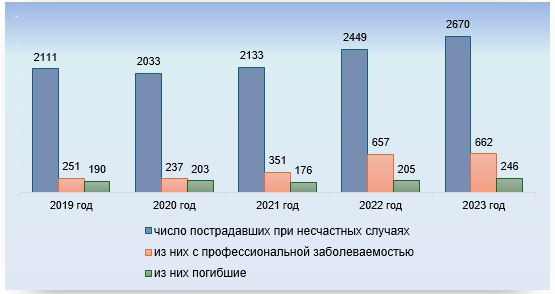
\includegraphics[width=0.7\textwidth]{media/ekon/image5.1}
	\caption*{Рис. 1 - Динамика числа пострадавших и погибших при НСТ, чел.}
  \emph{Примечание -- составлено авторами на основании статистических
  данных {[}15{]}}
\end{figure}

\begin{multicols}{2}


  Количество погибших в результате несчастных случаев, связанных с
  трудовой деятельностью в 2023 году составило 246 человек, 2019 году этот
  показатель был равен 190 человек, рост составил 29,5\%. Наблюдается
  значительный рост числа пострадавших за последние пять лет. Если в 2019
  году количество пострадавших составляло 2111 человек, то в 2023 году оно
  достигло 2670 человек, что соответствует росту на 26,5\%. Это указывает
  на увеличение частоты или тяжести несчастных случаев на производстве.
  исло людей с выявленными профессиональными заболеваниями также возросло,
  увеличившись с 251 случая в 2019 году до 662 случаев в 2023 году. Это
  увеличение в 1,6 раза свидетельствует о неблагоприятных условиях труда,
  которые могут требовать дополнительных мер профилактики и реабилитации
  (рисунок 1).

Рисунок 1 показывает рост всех трех показателей -пострадавших,
профессиональной заболеваемости и погибших - указывает на ухудшение
условий труда или недостаточность мер, направленных на их улучшение.
Увеличение профессиональной заболеваемости особенно подчеркивает
важность профилактики и улучшения медицинского обслуживания для
работников во вредных условиях. Эти данные подчеркивают необходимость
внедрения человекоцентричного подхода, при котором государство и
работодатели будут стремиться не только к компенсации последствий, но и
к активной профилактике профессиональных рисков. Человекоцентричный
подход может включать регулярные медицинские осмотры, улучшение условий
труда и систематическую оценку рабочих процессов для минимизации
профессиональных заболеваний и несчастных случаев.

Распределение производственных травм и смертности среди различных
профессиональных групп подчеркивает необходимость целенаправленных мер
по обеспечению безопасности труда и социальной защиты, учитывающих
специфику каждого вида деятельности. В условиях, когда одни категории
работников сталкиваются с гораздо более высокими уровнями риска, чем
другие, важно формировать человекоцентричную систему социальных
гарантий, способную гибко реагировать на потребности каждой группы.
Такой подход не только позволяет минимизировать последствия несчастных
случаев, но и направлен на создание устойчивых и безопасных условий
труда, особенно для тех категорий, где профессиональные риски наиболее
высоки.

Вышесказанное подтверждается данными, представленными на рисунке 2, где
отражено распределение числа пострадавших и погибших по профессиональным
группам. Эти данные демонстрируют существенные различия в уровне
травматизма и смертности в зависимости от сферы деятельности,
подчеркивая необходимость дифференцированного подхода к вопросам
безопасности и социальных гарантий. Человек, работающий в условиях
повышенного риска, требует особой поддержки и защиты, что делает
человекоцентричный подход особенно актуальным в контексте снижения
профессиональных рисков и повышения качества условий труда.


Принцип человекоцентричности подразумевает ориентацию на человека как на
центральное звено всех процессов и систем {[}16{]}.Человек в центре
системы управления --- это не просто лозунг, а комплексный подход,
который предполагает обеспечение здоровья, безопасности,
удовлетворенности и социальной защищенности работников. В этом контексте
социальные гарантии выступают важнейшим элементом человекоцентричной
модели, так как они непосредственно направлены на поддержание качества
жизни и благополучия человека. Социальные гарантии включают не только
выплаты и компенсации, но также меры по охране здоровья, реабилитации,
профессиональной поддержке и развитию, что позволяет работникам
чувствовать себя более защищенными и уверенными в стабильности своего
положения.

В Казахстане принимаются последовательные меры по продвижению принципов
концепции достойного труда путем совершенствования национального
законодательства, в том числе путем внедрения в него международных норм.
Так, в 2023 году в Казахстане был принят новый Социальный кодекс, в
рамках которого были пересмотрены подходы к социальной защите населения,
внесены изменения и дополнения в Трудовой кодекс, направленные на
укрепление социального диалога и институционального потенциала
социальных партнеров и др.

\end{multicols}


\begin{figure}[H]
	\centering
	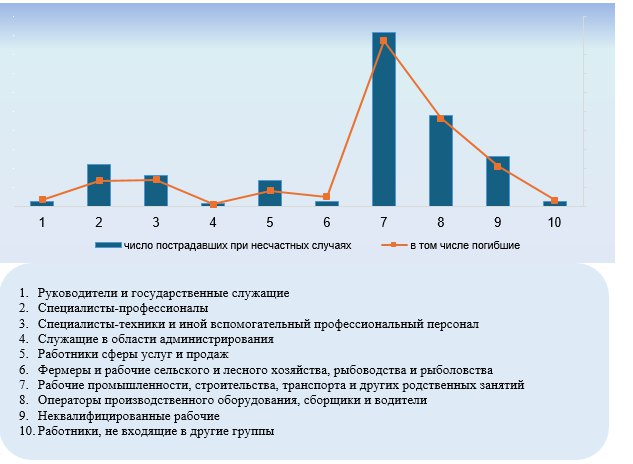
\includegraphics[width=0.8\textwidth]{media/ekon/image5.2}
	\caption*{Рис. 2 - Анализ числа пострадавших и погибших при НСТ по роду
  деятельности (в среднем за 2019--2023 гг.), чел.}
  \emph{Примечание -- составлено авторами на основании статистических
  данных {[}15{]}}
\end{figure}

\begin{multicols}{2}

Реализация принципов Достойного труда закреплена в Генеральном
соглашении на 2024-2026 годы, подписанном в марте 2024 года между
Правительством РК, республиканскими объединениями профсоюзов и
республиканскими объединениями работодателей. В рамках Генерального
соглашения социальные партнеры приняли совместные обязательства,
направленные на создание качественных рабочих мест, предусматривающих
безопасные условия труда, достойную оплату, социальные гарантии, доступ
к обучению и повышению квалификации и т.д.

Система социальных гарантий и компенсаций для работников во вредных
условиях в Республике Казахстан направлена на комплексную поддержку: от
финансовых доплат и дополнительного отдыха до специальных мер в виде
лечебного питания и сокращенного рабочего времени. Эта структура
свидетельствует о человекоцентричном подходе к защите здоровья
работников, так как охватывает как финансовые, так и профилактические
меры для минимизации негативного воздействия неблагоприятных условий
труда (рисунок 3).

Однако, несмотря на комплексность структуры компенсаций за работу во
вредных условиях в Казахстане, практика показывает, что в ряде других
стран к подобным мерам применяются еще более углубленные и
специализированные подходы, ориентированные на долгосрочное здоровье
работников и более высокий уровень социальной защиты.

В современных условиях экономика требует пересмотра роли государства в
системе управления охраной труда. Государство сохраняет функцию гаранта
прав работников на труд в безопасных и гигиеничных условиях, что
закрепляется соответствующей нормативно-правовой базой. При этом
формирование безопасных условий труда остается задачей самих
предприятий. Основные решения в этой сфере принимаются руководством
компаний, а мотивация предприятий чаще всего носит экономический
характер.

\end{multicols}


\begin{figure}[H]
	\centering
	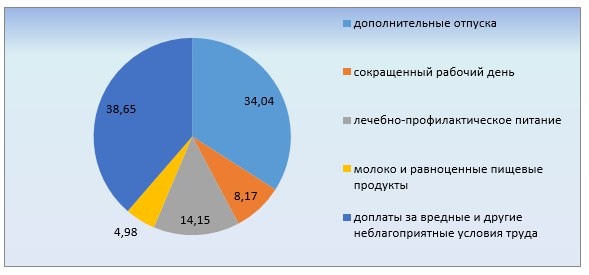
\includegraphics[width=0.8\textwidth]{media/ekon/image5.3}
	\caption*{Рис. 3 -- Структура компенсаций за работу во вредных и других
  неблагоприятных условиях труда}
  \emph{Примечание -- составлено авторами на основании статистических
  данных {[}15{]}}
\end{figure}

\begin{multicols}{2}


Анализ структуры экономических затрат предприятий позволяет глубже
понять их поведение и выработать правила, способные эффективно влиять на
процесс принятия решений. Одним из индикаторов, отражающих затраты,
являются материальные последствия несчастных случаев на производстве
(МП-НСТ), которые представлены в денежном выражении и включают:

\begin{itemize}
\item
  суммы, выплаченные по листку нетрудоспособности;
\item
  суммы доплат до прежнего заработка при переводе на другую работу;
\item
  суммы единовременных пособий.
\end{itemize}

Данный показатель анализируется в разрезе видов экономической
деятельности и регионов Республики Казахстан. Динамика МП-НСТ за
2014--2023 годы демонстрирует ежегодный рост, несмотря на снижение числа
несчастных случаев. Особенно заметный скачок наблюдается в 2022 году,
когда показатель увеличился более чем в два раза, достигнув 4,1 млрд
тенге, а в 2023 году вырос еще на 98\%, составив 8,1 млрд тенге. Такой
рост может быть связан с увеличением уровня заработных плат, пересмотром
сумм компенсаций и увеличением расходов на единовременные выплаты.

Данные, представленные в таблице 1, показывают структуру МП-НСТ за
2020--2023 годы.


Из представленных данных следует, что основная доля затрат приходится на
единовременные пособия, которые за 2023 год составили 62,3\% от общей
суммы. Выплаты по листку нетрудоспособности варьируются от 36,3\% до
45,9\%, тогда как доплаты до прежнего заработка занимают менее 2\%.
Прирост показателей за последние три года демонстрирует их
нестабильность. Так, за период с 2021 по 2023 годы выплаты по листкам
нетрудоспособности выросли на 60\% и 58\% ежегодно, а доплаты при
переводе на другую работу увеличились на 145\% и 394\% соответственно.


Полученные результаты свидетельствуют о необходимости пересмотра
существующих подходов к управлению охраной труда. Основной акцент должен
быть сделан на внедрение человекоцентричных подходов, которые
предполагают приоритетное внимание к потребностям работников, их
здоровью и благополучию. Профилактические меры, такие как улучшение
условий труда, регулярные медицинские осмотры и программы по обучению
безопасному поведению, должны стать неотъемлемой частью системы
управления. Такой подход не только способствует снижению травматизма и
связанных с ним затрат, но и повышает удовлетворенность работников, их
вовлеченность и лояльность, что в долгосрочной перспективе положительно
сказывается на эффективности предприятий.
\end{multicols}

\begin{longtable}[H]{|@{} 
  >{\raggedright\arraybackslash}p{(\columnwidth - 8\tabcolsep) * \real{0.1009}}| 
  >{\raggedright\arraybackslash}p{(\columnwidth - 8\tabcolsep) * \real{0.2819}}| 
  >{\raggedright\arraybackslash}p{(\columnwidth - 8\tabcolsep) * \real{0.2819}}| 
  >{\raggedright\arraybackslash}p{(\columnwidth - 8\tabcolsep) * \real{0.1274}}| 
  >{\raggedright\arraybackslash}p{(\columnwidth - 8\tabcolsep) * \real{0.2079}}|@{}}
  \caption*{Таб. 1 -- Структура материальных последствий несчастных случаев
  на производстве}\\
  \hline
\begin{minipage}[b]{\linewidth}\raggedright
Год
\end{minipage} & \begin{minipage}[b]{\linewidth}\raggedright
Материальные последствия НСТ, всего (тыс. тенге)
\end{minipage} & \begin{minipage}[b]{\linewidth}\raggedright
Выплаты по листку нетрудоспособности
\end{minipage} & \begin{minipage}[b]{\linewidth}\raggedright
Доплаты до прежнего заработка
\end{minipage} & \begin{minipage}[b]{\linewidth}\raggedright
Единовременные пособия
\end{minipage} \\ 
\endhead
\endfoot
\hline
2020 & 1 971 764 & 45,90\% & 0,30\% & 53,80\% \\
2021 & 2 636 723 & 44,10\% & 0,40\% & 55,50\% \\
2022 & 4 106 739 & 45,40\% & 0,60\% & 54,00\% \\
2023 & 8 134 962 & 36,30\% & 1,40\% & 62,30\% \\
\hline
\multicolumn{5}{|@{}>{\raggedright\arraybackslash}p{(\columnwidth - 8\tabcolsep) * \real{1.0000} + 8\tabcolsep}|@{}}{%
\emph{Примечание -- составлено авторами на основании статистических
данных {[}15{]}}} \\ \hline
\end{longtable}

\begin{multicols}{2}

Так, например, в Германии система компенсаций для работников, занятых во
вредных условиях труда, включает не только дополнительные отпуска и
доплаты, но и обязательное предоставление медицинской страховки,
покрывающей специализированное обследование и лечение профессиональных
заболеваний. Более того, немецкие компании обязаны проводить регулярные
тренинги по охране труда и безопасности, что способствует снижению
производственного травматизма и повышению осведомленности сотрудников о
возможных рисках.

В Норвегии, которая известна своим высоким уровнем социальной защиты,
работники, занятые на опасных производствах, получают компенсации в виде
пенсионных льгот, позволяющих им выходить на пенсию раньше. Также в
Норвегии активно развиваются программы профилактической медицины,
включающие бесплатное санаторно-курортное лечение для сотрудников,
подверженных воздействию вредных факторов на рабочем месте. Такие
программы позволяют минимизировать долгосрочные последствия для здоровья
работников и способствуют продлению их трудовой активности.

В Японии для работников, занятых во вредных условиях, помимо стандартных
компенсаций, предоставляются уникальные программы психологической
поддержки, так как в японской культуре работа на опасных производствах
часто сопряжена с высоким уровнем стресса. Работники имеют доступ к
бесплатным консультациям психологов и специальным программам снижения
стресса, что помогает снизить не только физическую, но и
психоэмоциональную нагрузку на них.

Международной организации труда (МОТ) подчеркивается, что инвестиции в
улучшение условий труда и здоровья работников окупаются за счет
сокращения числа несчастных случаев и связанных с ними затрат. Так,
согласно данным МОТ, каждое вложенное в охрану труда евро возвращает от
2 до 5 евро за счет снижения производственных рисков и повышения
эффективности работы\hspace{0pt}\hspace{0pt}. Примером успешного
внедрения таких мер является опыт стран Европейского Союза. В Швеции
реализация профилактических программ позволила сократить
производственный травматизм на 25\% за последние 10 лет. Аналогичные
результаты достигнуты в Германии, где внедрение программ по реабилитации
работников, пострадавших на производстве, позволило снизить общие
затраты работодателей на компенсации и выплаты на
30\%\hspace{0pt}\hspace{0pt}.

Кроме того, данные исследования, проведенного в Великобритании,
показывают, что инвестиции в программы обучения работников вопросам
безопасности труда снизили уровень травматизма на 40\% за пять лет. Эти
меры включали регулярные тренинги, улучшение условий труда и
предоставление дополнительных социальных льгот\hspace{0pt}.

Примеры из международной практики свидетельствуют, что ключевыми
факторами эффективности являются:

\begin{itemize}
\item
  акцент на профилактические меры;
\item
  вовлечение работников в разработку и реализацию программ охраны труда;
\item
  регулярный мониторинг и анализ показателей состояния здоровья
  сотрудников.
\end{itemize}

Таким образом, международный опыт подтверждает, что человекоцентричный
подход к социальной защите работников является не только этически
оправданным, но и экономически целесообразным.

{\bfseries Выводы.} Внедрение человекоцентричного подхода в систему
социальных гарантий для работников, занятых на опасных и вредных
производствах, предполагает переход от стандартного набора
компенсационных мер к более комплексной и гибкой системе поддержки,
ориентированной на потребности человека. Это требует пересмотра и
адаптации текущих мер социальной защиты, которые должны включать не
только компенсации за вредные условия, но и превентивные и
реабилитационные меры, способствующие улучшению здоровья и снижению
профессиональных рисков.

\emph{1. Усиление профилактических мер и охрана здоровья.}

Один из ключевых аспектов человекоцентричного подхода --- акцент на
профилактике профессиональных заболеваний и защите здоровья работников.
Для этого необходимо:

- регулярные углубленные медицинские осмотры. Медицинские обследования
работников, занятых во вредных условиях, должны проводиться чаще и
включать более широкий спектр анализов и диагностических мероприятий для
своевременного выявления профессиональных заболеваний;

\begin{itemize}
\item
  профилактические и оздоровительные программы. Государство и
  работодатели могут инвестировать в программы профилактики, которые
  позволят снижать воздействие вредных факторов на здоровье работников.
  Это может включать регулярное санаторно-курортное лечение и физическую
  реабилитацию;
\item
  программы психологической поддержки. Вредные условия труда зачастую
  сопровождаются высоким уровнем стресса, что может оказывать негативное
  влияние на психическое здоровье работников. Важно развивать программы
  психологической поддержки, которые помогут минимизировать стресс и
  улучшить общее состояние работников.
\end{itemize}

\emph{2. Индивидуализированные компенсационные и реабилитационные
пакеты.}

Человекоцентричный подход требует адаптации социальной защиты к
индивидуальным потребностям работников. Для этого могут быть внедрены
следующие меры:

\begin{itemize}
\item
  индивидуальные компенсационные пакеты. Для каждого работника
  необходимо разрабатывать адаптированные пакеты социальной поддержки.
  Это может включать дополнительное страхование, покрытие затрат на
  медицинские услуги, поддержку в лечении хронических заболеваний,
  связанных с условиями труда;
\item
  реабилитационные программы. Работникам, которые пострадали на
  производстве или приобрели профессиональные заболевания, должны
  предоставляться широкие возможности для реабилитации, включая
  поддержку в восстановлении после травм и болезней, связанных с
  производством.
\end{itemize}

\emph{3. Участие работников в принятии решений о социальных гарантиях}

Эффективное внедрение человекоцентричного подхода требует учета мнения
самих работников при формировании социальной политики. Это можно
реализовать через:

\begin{itemize}
\item
  создание консультативных советов или комитетов по охране труда.
  Работники, занятые во вредных условиях, могут активно участвовать в
  обсуждении мер безопасности и социальной поддержки. Это обеспечит,
  чтобы принятые решения реально отвечали потребностям тех, кто
  находится в зоне риска;
\item
  регулярное проведение опросов и сбор обратной связи. Это поможет
  понять, насколько эффективно работают текущие социальные гарантии и
  какие улучшения требуются с точки зрения самих сотрудников.
\end{itemize}

\emph{4. Улучшение условий труда через инновации и модернизацию
оборудования.}

Для снижения уровня травматизма и профессиональной заболеваемости
необходимо внедрять инновационные технологии и модернизировать
оборудование. Это может включать:

\begin{itemize}
\item
  автоматизацию и роботизацию процессов. Во многих случаях внедрение
  автоматизированных систем может снизить необходимость участия
  работников в наиболее опасных производственных процессах;
\item
  обновление оборудования и обеспечение дополнительными средствами
  защиты. Устаревшее оборудование часто является причиной травм и
  профессиональных заболеваний. Внедрение современного, более
  безопасного оборудования --- одна из ключевых мер человекоцентричного
  подхода.
\end{itemize}

\emph{{\bfseries Финансирование}. В статье представлены результаты
исследования, полученные в ходе реализации научно-технической программы
«Трансформация государственного механизма социальных гарантий в
отношении лиц, занятых во вредных условиях труда, в современных
условиях» (ИРН BR22182673).}


\end{multicols}
\begin{center}

{\bfseries Литература}
\end{center}
\begin{references}

\begin{enumerate}
\def\labelenumi{\arabic{enumi}.}
\item
  Концепция развития государственного управления в Республике Казахстан
  до 2030 года - \linebreak {https://adilet.zan.kz/rus/docs/U2100000522}
\item
  Гальченко С.А., Сезонова О.Н., Ходыревская В.Н., Трубникова В.В.,
  Рюмшин А.В. Человекоцентричность -- необходимое условие экономики
  будущего // Лидерство и менеджмент. -2022.- Том 9.- № 2.- С. 309-322.
  DOI 10.18334/lim.9.2.114587.
\item
  Абдешов Д.Д., Косумбаева Ш.И., Салкынбаева Ф.Д. Человекоцентричная
  модель управления человеческими ресурсами. Вестник науки. 2024. №5
  (74). С. 37--40.
\item
  Министерство труда и социальной защиты населения Республики Казахстан.
  (2022). Охрана труда в Республике Казахстан: Национальный обзор.
  Астана: Республиканский научно-исследовательский институт по охране
  труда, 2022.-146 стр.
  \href{https://www.kazenergy.com/upload/document/development/ohrana_2023.pdf}{https://www.kazenergy.com}
\item
  Ш.К. Абикенова, А.П. Коваль, Л.М. Шаяхметова, А.Б. Бекмагамбетов, Ш.Т.
  Айтимова Современные условия труда, уровень производственного
  травматизма на основе данных национальной статистики и других
  источников информации: ЗН РК. «Вестник НАН РК», 403(3), 281--297.

  \href{https://doi.org/10.32014/2023.2518-1467.509}{DOI
  10.32014/2023.2518-1467.509}
\item
  Ш.К. Абикенова, Г. А. Еселханова, Ж. Х. Есбенбетова Доплата за вредные
  условия труда//Охрана здоровья и окружающей среды. -- 2016.-№ 9 -
  https://e.otruda.mcfr.kz/496017
\item
  Д.М. Турекулова, Б.Т. Череева, Е.С. Петренко Совершенствование
  организации охраны и безопасности труда на производстве//Экономическая
  серия Вестника ЕНУ им. Л.Н. Гумилева.- 2023.- №.-C. 77 -85 DOI:
  {https://doi.org/10.32523/2789-4320-2023-2-77-85}
\item
  А.Б. Бекмагамбетов Право на безопасные условия труда в Республике
  Казахстан: совершенствование экономико-правового механизма// Вестник
  ЮУрГУ. Серия «Право».- 2022.- Т. -22.- № 3.- С. 55-- 60. DOI:
  10.14529/law220308
\item
  International Labour Organization (ILO). (2001). Guidelines on
  occupational safety and health management systems (ILO-OSH 2001).
  Geneva: ILO. \href{https://www.ilo.org/global/topics/safety-and-health-at-work/WCMS\_107727/lang-\/-en/index.htm}{https://www.ilo.org}
\item
  International Organization for Standardization (ISO). (2018). ISO
  45001:2018 -- Occupational health and safety management systems --
  Requirements with guidance for use. Geneva: ISO.
  \linebreak {https://www.iso.org/standard/63787.html}
\item
  Сергунина Н.А., Быкова Н. Москва: умные решения для качества жизни.
  Стандарты и качество. -- 2021.- № 10. - С. 84--87.
  https://elibrary.ru/item.asp?id=46943543
\item
  Жагловская А.В. Концепция человекоцентричных предприятий в отраслевой
  экономике: имущественный аспект//Вестник Евразийской науки.- 2023.- Т.
  15( 6).- С.1-9 
  
  URL: https://esj.today/PDF/67ECVN623.pdf
\item
  Жагловская, А.В. Концепция человекоцентричных предприятий в отраслевой
  экономике: имущественныйаспект / А. В. Жагловская // Вестник
  евразийской науки.- 2023.- -Т.15. - № 6.
  \linebreak {URL:https://esj.today/PDF/67ECVN623.pdf}
\item
  Насырова С.И. Межкомпонентные отношения в экономике, ориентированной
  на человека (часть первая) // Экономика и управление. - 2021.-№
  8(190).- С. 612-621.DOI 10.35854/1998--1627--2021--8-612--621.
\item
  О травматизме, связанном с трудовой деятельностью, и профессиональных
  заболеваниях в Республике Казахстан за 2021 год -
  \href{https://stat.gov.kz/ru/industries/social-statistics/stat-medicine/publications/3965/}{https://stat.gov.kz}
\item
  Искендирова, С., Дауешова, А., \& Амирова , А. . (2024). Экосистемный,
  цифровой и человекоцентричный подход на государственной службе:
  международный опыт и возможности для Казахстана. Государственное
  управление и государственная служба.- 2024.-№ 3(90).-С. 150-159.
  \linebreak {https://doi.org/10.52123/1994-2370-2024-1317}
\end{enumerate}
\end{references}
\begin{center}

{\bfseries References}

\end{center}
\begin{references}
\begin{enumerate}
\def\labelenumi{\arabic{enumi}.}
\item
  Koncepcija razvitija gosudarstvennogo upravlenija v Respublike
  Kazahstan do 2030 goda -
  \linebreak {https://adilet.zan.kz/rus/docs/U2100000522}. {[}in Russian{]}
\item
  Abdeshov D.D., Kosumbaeva Sh.I., Salkynbaeva F.D.
  Chelovekocentrichnaya model upravleniya \\chelovecheskimi resursami.
  Vestnik nauki. 2024. №5 (74). S. 37--40. {[}in Russian{]}
\item
  Gal' chenko S.A., Sezonova O.N., Hodyrevskaja V.N.,
  Trubnikova V.V., Rjumshin A.V. \\Chelovekocentrichnost'{}
  -- neobhodimoe uslovie jekonomiki budushhego // Liderstvo i
  menedzhment. -2022.- Tom 9.- № 2.- S. 309-322. DOI
  10.18334/lim.9.2.114587. {[}in Russian{]}
\item
  Ministerstvo truda i social' noj zashhity naselenija
  Respubliki Kazahstan. (2022). Ohrana truda v Respublike Kazahstan:
  Nacional' nyj obzor. Astana: Respublikanskij
  nauchno-issledovatel' skij institut po ohrane truda,
  \href{https://www.kazenergy.com/upload/document/development/ohrana_2023.pdf}{https://www.kazenergy.com}
  2022.-146 str.  {[}in Russian{]}
\item
  Sh.K. Abikenova, A.P. Koval', L.M. Shajahmetova, A.B.
  Bekmagambetov, Sh.T. Ajtimova Sovremennye uslovija truda,
  uroven'{} proizvodstvennogo travmatizma na osnove
  dannyh nacional' noj statistiki i drugih istochnikov
  informacii: ZN RK. «Vestnik NAN RK», 403(3), 281--297. DOI
  10.32014/2023.2518-1467.509 {[}in Russian{]}
\item
  Sh.K. Abikenova, G. A. Eselhanova, Zh. H. Esbenbetova Doplata za
  vrednye uslovija truda//Ohrana zdorov' ja i
  okruzhajushhej sredy. -- 2016.-№ 9 -
  {https://e.otruda.mcfr.kz/496017}{[}in Russian{]}
\item
  D.M. Turekulova, B.T. Chereeva, E.S. Petrenko Sovershenstvovanie
  organizacii ohrany i bezopasnosti truda na
  proizvodstve//Jekonomicheskaja serija Vestnika ENU im. L.N. Gumileva.-
  2023.- №.-C. 77 -85 DOI:
  {https://doi.org/10.32523/2789-4320-2023-2-77-85} {[}in Russian{]}
\item
  A.B. Bekmagambetov Pravo na bezopasnye uslovija truda v Respublike
  Kazahstan: sovershenstvovanie jekonomiko-pravovogo mehanizma// Vestnik
  JuUrGU. Serija «Pravo».- 2022.- T. -22.- № 3.- S. 55-- 60. DOI:
  10.14529/law220308. {[}in Russian{]}
\item
  International Labour Organization (ILO). (2001). Guidelines on
  occupational safety and health management systems (ILO-OSH 2001).
  Geneva: ILO.\href{https://www.ilo.org/global/topics/safety-and-health-at-work/WCMS\_107727/lang-\/-en/index.htm}{https://www.ilo.org}
\item
  International Organization for Standardization (ISO). (2018). ISO
  45001:2018 -- Occupational health and safety management systems --
  Requirements with guidance for use. Geneva: ISO.
  \linebreak {https://www.iso.org/standard/63787.html}
\end{enumerate}

11. Sergunina N.A., Bykova N. Moskva: umnye reshenija dlja kachestva
zhizni. Standarty i kachestvo. -- 2021.- № 10. - S. 84--87.
https://elibrary.ru/item.asp?id=46943543 {[}in Russian{]}

12. Zhaglovskaja A.V. Koncepcija chelovekocentrichnyh predprijatij v
otraslevoj jekonomike: \linebreak imushhestvennyj aspekt//Vestnik Evrazijskoj
nauki.- 2023.- T. 15( 6).- S.1-9. \linebreak URL:
{https://esj.today/PDF/67ECVN623.pdf}. {[}in Russian{]}

13. Zhaglovskaja, A.V. Koncepcija chelovekocentrichnyh predprijatij v
otraslevoj jekonomike: \linebreak imushhestvennyjaspekt / A. V. Zhaglovskaja //
Vestnik evrazijskoj nauki.- 2023.- -T.15. - № 6.
\linebreak {URL:https://esj.today/PDF/67ECVN623.pdf}. {[}in Russian{]}

14. Nasyrova S.I. Mezhkomponentnye otnoshenija v jekonomike,
orientirovannoj na cheloveka (chast'{} pervaja) //
Jekonomika i upravlenie. - 2021.-№ 8(190).- S. 612-621.DOI
10.35854/1998--1627--2021--8-612--621. {[}in Russian{]}


15. O travmatizme, svjazannom s trudovoj
dejatel' nost' ju, i
professional' nyh zabolevanijah v Respublike Kazahstan za
2021 god -
https://stat.gov.kz/ru/industries/social-statistics/stat-medicine/publications/3965/
{[}in Russian{]}

16. Iskendirova, S., Daueshova, A., \& Amirova , A. . (2024).
Jekosistemnyj, cifrovoj i chelovekocentrichnyj podhod na gosudarstvennoj
sluzhbe: mezhdunarodnyj opyt i vozmozhnosti dlja Kazahstana.
Gosudarstvennoe upravlenie i gosudarstvennaja sluzhba.- 2024.-№
3(90).-S. 150-159. {https://doi.org/10.52123/1994-2370-2024-1317}
{[}in Russian{]}
\end{references}
\begin{authorinfo}

  \hspace{1em}\emph{{\bfseries Сведения об авторах}}

Курманов А.М.- к.э.н.,генеральный директор «Республиканского
научно-исследовательского института охраны труда и здоровья Министерства
труда и социальной защиты населения Республики Казахстан», Астана,
Казахстан, e-mail: rniiot@rniiot.kz;

Бекмагамбетов А.Б - к.ю.н., ассоциированный профессор, заместитель
генерального директора Республиканского научно-исследовательский
институт по охране труда Министерства труда и социальной защиты
населения Республики, Астана, Казахстан, e-mail:
\href{mailto:adilet1979@mail.ru}{\nolinkurl{adilet1979@mail.ru}};

Сарыбаева И.Е. - докторант Евразийского национального университета имени
Л.Н. Гумилева, Астана, Казахстан, e-mail: inarasaribaeva@gmail.com;

Енсебаева А.Р. - к.ю.н., руководитель отдела социально-правовых
исследований «Республиканского научно-\\исследовательского института
охраны труда и здоровья Министерства труда и социальной защиты населения
Республики Казахстан», Астана, Казахстан, е-mail:
\href{mailto:nel1212kz@gmail.com}{\nolinkurl{nel1212kz@gmail.com}};

Омаркожаева А.Н. - к.э.н., доцент, ведущий научный работник Проекта,
Астана, Казахстан, e-mail: asya\_7510@mail.ru

\hspace{1em}\emph{{\bfseries Information about the authors}}

Kurmanov A.M. - Candidate of Economic Sciences, General Director,
`Republican Research Institute of Labour Protection and Health of the
Ministry of Labour and Social Protection of the Population of the
Republic of Kazakhstan' (Astana, Kazakhstan), е-mail: rniiot@rniiot.kz;

Bekmagambetov A.B. - Candidate of Law, Associate Professor, Deputy
Director General of the Republican Research Institute of Labour
Protection and Health of the Ministry of Labour and Social Protection of
the Republic of Kazakhstan, Astana, Kazakhstan, е-mail:
\href{mailto:adilet1979@mail.ru}{\nolinkurl{adilet1979@mail.ru}};

Sarybaeva I.E. - doctoral student, L.N. Gumilev Eurasian National
University, Astana, Kazakhstan, \\е-mail: inarasaribaeva@gmail.com;

Yensebayeva A.R. - Candidate of Law, Head of the Department of Social
and Legal Research `Republican Research Institute of Labour Protection
and Health of the Ministry of Labour and Social Protection of the
Population of the Republic of Kazakhstan', Astana, Kazakhstan, e-mail:
nel1212kz@gmail.com;

Omarkozhaeva A.N. - Candidate of е-mail: Economic Sciences, Associate
Professor, Leading Researcher of the Project, Astana, Kazakhstan,
e-mail: asya\_7510@mail.ru.
\end{authorinfo}
